\documentclass[%
reprint,
%superscriptaddress,
%groupedaddress,
%unsortedaddress,
%runinaddress,
%frontmatterverbose, 
%preprint,
%preprintnumbers,
%nofootinbib,
%nobibnotes,
%bibnotes,
 amsmath,amssymb,
 aps,
%pra,
%prb,
%rmp,
%prstab,
%prstper,
%floatfix,
]{revtex4-2}

\usepackage{subfiles}
\usepackage{graphicx}% Include figure files
\usepackage{dcolumn}% Align table columns on decimal point
\usepackage{bm}% bold math
\usepackage{float}
\usepackage{mathtools}
\usepackage{physics}
\usepackage{tcolorbox}
\usepackage{tensor}
%\usepackage{hyperref}% add hypertext capabilities
%\usepackage[mathlines]{lineno}% Enable numbering of text and display math
%\linenumbers\relax % Commence numbering lines

%\usepackage[showframe,%Uncomment any one of the following lines to test 
%%scale=0.7, marginratio={1:1, 2:3}, ignoreall,% default settings
%%text={7in,10in},centering,
%%margin=1.5in,
%%total={6.5in,8.75in}, top=1.2in, left=0.9in, includefoot,
%%height=10in,a5paper,hmargin={3cm,0.8in},
%]{geometry}

\newcommand{\Hp}{\mathcal{H}}

\begin{document}

\section{Evolution of structure in the Universe}
\label{sec:3}
The topic of this section is to see how small quantum fluctuations from the inflationary period caused small perturbations to the baryon, photon and dark matter fluid in the early which then grew into large structures formations we see today. Since we have determined various quantities of the background cosmology in the previous sections, all we need to do is to perturb the background and determine suitable initial conditions. To do this we write the perturbed flat FRLW metric in the Newtonian gauge. Note that from this section and onwards we set $N_\text{eff}=0$, completely neglecting neutrinos from hereon.

\subsection{Theory}
\subsubsection{Metric perturbations}
As mentioned in the intro we consider perturbations to the flat FLRW metric:
\[g_{\mu\nu}=g^{0}_{\mu\nu}+h_{\mu\nu},\quad\quad|h_{\mu\nu}|\ll1,\]
where $g^0_{\mu\nu}$ is the pure FLRW metric and $h_{\mu\nu}$ is a small perturbation. By $|h_{\mu\nu}|\ll1$ we mean that there exists some coordinate system where the components of $h_{\mu\nu}$ satisfy this. The Newtonian gauge in Cartesian coordinates is defined by
\[h_{00}=-2\Psi,\quad h_{0i}=0,\quad h_{ij}=2a^2\delta_{ij}\Phi,\]
where $\Psi=\Psi(t,\textbf{x})$ and $\Phi=\Phi(t,\textbf{x})$ are scalar perturbations of the flat FRLW metric which happen to be the Newtonian potential and the Newtonian curvature respectively. Note that this implies $\Psi\ll1$ and $\Phi\ll 1$. As such the line element in Cartesian coordinates and the Newtonian gauge takes the form
\[ds^2=-(1+2\Psi)dt^2+a^2(t)(1+2\Phi)d\textbf{x}^2.\]
\subsubsection{Photon temperature fluctuations}
Since we are interested in solving perturbations to the Boltzmann equations for the various particle types we first consider the Boltzmann equation for photons:
\[\frac{df}{dt}=C[f],\]
where $f=f(\textbf{x},\textbf{p},t)$ is the Bose-Einstein distribution due to photons being relativistic integer spin particles and $C[f]$ is the collision term due to Thompson scattering. Expanding the total derivative on the left via the chain rule yields:
\begin{equation}
	\frac{df}{dt}=\pdv{f}{t}+\pdv{f}{\textbf{x}}\frac{d\textbf{x}}{dt}+\pdv{f}{|\textbf{p}|}\frac{d|\textbf{p}|}{dt}+\pdv{f}{\hat{\textbf{p}}}\frac{d\hat{\textbf{p}}}{dt},
	\label{eq:collessBE}
\end{equation}
where $\hat{\textbf{p}}=\textbf{p}/|\textbf{p}|$ is the direction of the photon propagation. Using the geodesic equation and the metric whilst only keeping first order terms, one can show that (\ref{eq:collessBE}) can be rewritten to a more convenient form:
\begin{align*}
	\frac{df}{dt}=\pdv{f}{t}+\frac{p}{E}\frac{\hat{\textbf{p}}}{a}\pdv{f}{\textbf{x}}-|\textbf{p}|\pdv{f}{|\textbf{p}|}\left[H+\frac{d\Phi}{dt}+\frac{E}{a}\frac{\hat{\textbf{p}}}{|\textbf{p}|}\pdv{\Psi}{\textbf{x}}.\right]
\end{align*}
Since we know the CMB is roughly $T^{0}=2.7255\,$K with small fluctuations around this average, we then define the perturbation about this equilibrium:
\[T(\textbf{x},\hat{\textbf{p}},t)=T^{0}[1+\Theta(\textbf{x},\hat{\textbf{p}},t)].\]
One can show that all terms dependent on the magnitude of the momenta stemming from the Boltzmann equation for photons, can be rewritten in terms of $\Psi$ and $\Phi$ to first order.  As such the collision term for Thompson scattering in the Boltzmann equation then takes the form
\begin{equation}
	C[f(\textbf{p})]=-p\pdv{f^{0}}{p}n_e\sigma_T[\Theta_0-\Theta(\hat {\textbf{p}})+\hat{\textbf{p}}\cdot\textbf{v}_b],
	\label{eq:BEgammaR}
\end{equation}
where $\textbf{v}_b$ is the bulk velocity of baryons. A more in-depth derivation can be found in \cite{Dodelson:2003ft}. As mentioned in the prior section, we can ignore the contributions from protons as $m_p\gg m_e$ since the Thompson cross section $\sigma_T\propto m^{-2}$. Thus in practice it really only specifies the bulk velocity of electrons before recombination. The other side of the Boltzmann equation for photons to first order is:
\begin{equation}
	\frac{df}{dt}=-p\pdv{f^0}{p}\left[\pdv{\Theta}{t}+\frac{\hat{\textbf{p}}}{a}\pdv{\Theta}{\textbf{x}}+\frac{d\Phi}{dt}+\frac{\hat{\textbf{p}}}{a}\pdv{\Psi}{\textbf{x}} \right].
	\label{eq:BEgammaL}
\end{equation}
Equating (\ref{eq:BEgammaR}) and (\ref{eq:BEgammaL}) yields the Boltzmann equation for radiation to first order:
\begin{equation}
	\pdv{\Theta}{t}+\frac{\hat{\textbf{p}}}{a}\pdv{\Theta}{\textbf{x}}+\frac{d\Phi}{dt}+\frac{\hat{\textbf{p}}}{a}\pdv{\Psi}{\textbf{x}}=n_e\sigma_T[\Theta_0-\Theta(\hat {\textbf{p}})+\hat{\textbf{p}}\cdot\textbf{v}_b].
	\label{eq:BEgamma}
\end{equation}
Fourier transforming this and defining $\mu\equiv \hat{\textbf{p}}\cdot\textbf{k}/|\textbf{k}|$ where $\textbf{k}$ is the Fourier mode we can bring this into the form \cite{AST5220LectureNotes}
\begin{align}
	\pdv{\Theta}{t}+&\frac{ik\mu}{a}\Theta+\pdv{\Phi}{t}+\frac{ik\mu}{a}\Psi\nonumber\\
	&=n_e\sigma_T\left[\Theta_0-\Theta+i\mu v_b-\frac{P_2(\mu)}{2}\Theta_2\right],
	\label{eq:LOS_thingy}
\end{align}
where $P_2$ is the second order Legendre polynomial. We will come back to this last equation in section \ref{sec:4}.

\subsubsection{Matter density and velocity fluctuations}
Next we consider the Boltzmann equation for CDM. As mentioned in section \ref{sec:1} we consider CDM to be WIMPs, meaning their collision term is simply null. As mentioned earlier, CDM are non-relativistic particles, and thus their distribution function can be modelled as a Maxwell-Boltzmann distribution. Considering them to act as a perfect liquid and following a similar procedure one arrives at the cosmological generalization of the continuity equation and Euler equation respectively:
\begin{align}
	0&=\pdv{n}{t}+\frac{1}{a}\pdv{(n\textbf{v})}{\textbf{x}}+3n\left[H+\pdv{\Phi}{t}\right],
	\label{eq:contCDM}\\
	0&=\pdv{\textbf{v}}{t}+H\textbf{v}+\frac{1}{a}\pdv{\Psi}{\textbf{x}}.
\end{align}
Here we have suppressed the CDM label on the number density $n\equiv n_{\text{CDM}}$ and the bulk velocity $\textbf{v}\equiv \textbf{v}_\text{CDM}$ for readability. Further considering perturbations about the mean number density $n^0$:
\[n(\textbf{x},t)=n^0[1+\delta(\textbf{x},t)].\]
The first order contribution to (\ref{eq:contCDM}) is then
\begin{equation}
	\pdv{\delta}{t}+\frac{1}{a}\pdv{\textbf{v}}{\textbf{x}}+3\pdv{\Phi}{t}=0.
	\label{eq:delta_v_CDM}
\end{equation}
Baryons are also considered to behave as a non-relativistic fluid, meaning they satisfy Maxwell-Boltzmann distributions. The main difference between baryons and CDM is that they can interact amongst themselves and photons, the latter being via Thompson scattering. As mentioned in section \ref{sec:2}, Thompson scattering via protons can be neglected due to the cross section being inversely proportional to the square of the mass of the scattered particle. The perturbations to the cosmological continuity equation takes the same form as (\ref{eq:delta_v_CDM}), i.e.
\begin{equation}
	\pdv{\delta_\text{B}}{t}+\frac{1}{a}\pdv{\textbf{v}_\text{B}}{\textbf{x}}+3\pdv{\Phi}{t}=0.
	\label{eq:contB}
\end{equation}
However the corresponding Euler equation takes a different form due to interactions:
\begin{equation}
	\pdv{\textbf{v}_\text{B}}{t}+H\textbf{v}_\text{B}+\frac{1}{a}\pdv{\Psi}{\textbf{x}}=-n_e\sigma_T R(\textbf{v}_\gamma-\textbf{v}_\text{B}),
\end{equation}
where $R$ is defined in (\ref{eq:R}) and the parenthesis on the right hand side corresponds to the momentum transfer in the scattering process.
\subsubsection{Fourier transform and multipole expansions}
As of now all the relevant equation are all partial differential equations (PDEs) which remain tough to solve. Thus we wish to express these in terms of ODEs instead as this is something we know how to solve. We first consider the temperature perturbations $\Theta$. Since we are in general interested in the perturbations on various different scales in a mostly spherically symmetric universe we consider rewriting our functions in terms of multipole expansions. These are a series written in terms of Legendre polynomials $P_l(\zeta\equiv\cos\theta)$:
\[\Theta(t,k,\zeta)=\sum_{\ell=0}^\infty\frac{2\ell+1}{i^\ell}\Theta_\ell(t,k)P_\ell(\zeta).\]
The Legendre polynomials are orthonormal and form a complete basis. As such we can invert this equation in the same way as one would for Fourier coefficients to attain the Legendre multipoles:
\[\Theta_\ell(t,k)=\frac{i^\ell}{2}\int_{-1}^1d\zeta\, \Theta(t,k,\zeta)P_\ell(\zeta).\]
The most relevant moments are: the monopole $\Theta_0=\frac14\delta_\gamma$, the dipole $\Theta_1=-\frac13v_\gamma$ and the quadrupole $\Theta_2$. One can then recursively find all the Legendre polynomials by using Bonnet's recursion formula:
\[\zeta P_\ell=\frac{\ell+1}{2\ell+1}P_{\ell+1}+\frac{\ell}{2\ell+1}P_{\ell-1}.\]
Then, bringing (\ref{eq:BEgamma}) into Fourier space, switching to conformal time, using the above mentioned tricks together with the orthonormality of the Legendre polynomials, rewriting everything in terms of $x$, and reintroducing SI-units one find that the time dependence of the multipoles are given by:
\begin{align*}
	\Theta_0'&=-\frac{ck}{\Hp}\Theta_1-\Phi',\\
	\Theta_1'&=\frac{ck}{3\Hp}\Theta_0-\frac{2ck}{3\Hp}\Theta_2+\frac{ck}{3\Hp}\Psi+\tau'\left[\Theta_1+\frac{v_\text{B}}{3}\right],\\
	\Theta_\ell'&=\frac{\ell ck}{(2\ell+1)\Hp}\Theta_{\ell-1}-\frac{(\ell+1)ck}{(2\ell+1)\Hp}\Theta_{\ell+1},\\
	&+\tau'\left[\Theta_\ell-\frac{\Theta_\ell}{10}\delta_{\ell,2},\right],\quad\quad\ell\geq2,
\end{align*}
where the primes, as before, represent derivatives w.r.t. $x=\ln(a)$, $k$ is the corresponding Fourier coefficient and $v$ is defined via the relation $\textbf{v}=i\hat{\textbf{k}}v$.

Next we consider the scalar potentials $\Phi$ and $\Psi$ which can be found from the EFE. After some work one arrives at the following equations:
\begin{align*}
	\Phi'&=\Psi-\frac{1}{3}\left(\frac{ck}{\Hp}\right)^2\Phi+\frac{1}{2}\left[\delta\Omega_\text{CDM}+\delta_\text{B}\Omega_\text{B}+\delta_\gamma\Omega_\gamma\right],\\
	\Psi&=-\Phi-12\left(\frac{\Hp}{ck}\right)^2\Omega_\gamma\Theta_2.
\end{align*}
An in-depth derivation for this result can be seen in \cite{Dodelson:2003ft}.

Further, to simplify the problem of solving number density perturbations $\delta$ and bulk velocity $v$ for baryons and CDM we begin by expressing them in terms of conformal time and further translate them over to Fourier space to arrive at:
\begin{align*}
	\dot\delta&=-3\dot\Phi+kv,\\
	\dot v&=-k\Psi-\Hp v,\\
	\dot\delta_\text{B}&=-3\dot\Phi+kv_\text{B},\\
	\dot v_b&=-k\Psi+\dot\tau R(v_\text{B}-v_\gamma)-\Hp v_\text{B}.
\end{align*} 
As before we switch over to our time variable $x$ and use some of the relations between the multipoles. The results are summarized in equations (\ref{eq:photon_temp_multipoles}, \ref{eq:cdm_baryon_diffeqs}, \ref{eq:metric_perturbations_final}) where $\ell_\text{max}$ refers to the highest order multipole which we compute. 
\begin{tcolorbox}[
	width=\linewidth,
	colback=black!3!white,
	]
	\textbf{Photon temperature multipoles}
	\begin{subequations}\label{eq:photon_temp_multipoles}
		\begin{align}
			\Theta_0' &= -\frac{ck}{\Hp}\Theta_1-\Phi',
			\label{eq:photon_monopole}\\
			\Theta_1' &= \frac{ck}{3\Hp}\Theta_0 - \frac{2ck}{3\Hp}\Theta_2 +\frac{ck}{3\Hp}\Psi+\tau'\left[\Theta_1+\frac{1}{3}v_\text{B}\right],
			\label{eq:photon_dipole}\\
			\Theta_2'&=\frac{2ck}{5\Hp}\Theta_1-\frac{3ck}{5\Hp}\Theta_3+\frac{9}{10}\tau'\Theta_2,\\
			\Theta_\ell' &= \frac{\ell ck}{(2\ell+1)\Hp}\Theta_{\ell-1} -\frac{(\ell+1)ck}{(2\ell+1)\Hp}\Theta_{\ell+1} +\tau'\Theta_\ell,\\
			&\text{Above is valid for }2<\ell<\ell_\text{max},\nonumber\\
			\Theta_{\ell_{\text{max}}}' &=\frac{ck}{\Hp}\Theta_{\ell-1}-c\frac{\ell+1}{\Hp\eta}\Theta_\ell+\tau'\Theta_\ell.
		\end{align}
	\end{subequations}
	\\
	\textbf{CDM and baryons}
	\begin{subequations}\label{eq:cdm_baryon_diffeqs}
		\begin{align}
			\delta'&= \frac{ck}\Hp v-3\Phi',\\
			v'&= -v-\frac{ck}\Hp\Psi,\\
			\delta'_\text{B} &= \frac{ck}\Hp v_\text{B} - 3\Phi',\\
			v'_\text{B} &= -v_\text{B} - \frac{ck}\Hp\Psi + \tau'\,R(3\Theta_1+v_\text{B}).
		\end{align}
	\end{subequations}
	\\
	\textbf{Metric perturbations}
	\begin{subequations}\label{eq:metric_perturbations_final}
		\begin{align}
			\Phi' &= \Psi - \frac{c^2k^2}{3\Hp^2}\Phi + \frac{1}{2}[\delta\Omega_\text{CDM}+\delta_\text{B}\Omega_\text{B}+4\Omega_\gamma\Theta_0],\\
			\Psi &= -\Phi - \frac{12\mathcal{H}^2}{c^2k^2}\Omega_\gamma\Theta_2.
		\end{align}
	\end{subequations} 
\end{tcolorbox}
We have now removed all spatial dependency from the various quantities which are instead expressed in terms of the Fourier mode $k$. These modes now, instead of representing the spatial distribution, represent a unique spatial scale. Since Fourier modes in general are related to frequency, which is inversely proportional to wavelength, then $k\sim 1/\lambda$ where $\lambda$ is the relevant length scale. As such this is a very efficient way to look at what exactly happens at different cosmological scales. One can also relate these various scales to the Horizon to see what scales are causally connected and disconnected by considering the quantity $k\eta$. If $k\eta\gg1$ then we are working with scales much smaller than the horizon, if $k\eta\ll1$ these scales are much larger than the horizon and represent acausal distances. Finally $k\eta\simeq1$ is the scale at which the mode relates quantities which are the same magnitude as the horizon.


\subsubsection{Tight coupling}
One particular problem behind the set of differential equations in the very early Universe $\tau'\gg1$ due to photons and baryons being tightly coupled due to the primordial plasma, making it optically thick. $\tau\gg1$ implies that baryons in the early Universe only interacts with its close neighbourhood. This is what we call the \textbf{tight coupling regime}. This in turn causes the set of differential equations to be numerically unstable. To remedy this we instead attempt to consider a numerically stable approximation for $\Theta_1+\frac13v_\text{B}$ in this regime. Adding together $3\times$(\ref{eq:photon_dipole}) and (\ref{eq:cdm_baryon_diffeqs}d) yields
\begin{equation}
	[3\Theta_1+v_\text{B}]'=\frac{ck}{\Hp}(\Theta_0-2\Theta_2)+\tau'(1+R)[3\Theta_1+v_\text{B}]-v_\text{B}.
	\label{eq:3Tvb}
\end{equation}
Taking the next derivative of this, using $R'=-R$ and (\ref{eq:cdm_baryon_diffeqs}d) again to get rid of $-v_\text{B}'$ we arrive at
\begin{align*}
	[3\Theta_1+v_\text{B}]''=&-\frac{ck}{\Hp}\frac{\Hp'}{\Hp}(\Theta_0-2\Theta_2)+\frac{ck}{\Hp}(\Theta_0-2\Theta_2)'\\
	&+(\tau''(1+R)-R\tau')[3\Theta_1+v_\text{B}]\\
	&+(\tau'(1+R)-1)[3\Theta_1+v_\text{B}]'+3\Theta_1'.
\end{align*}
Substituting in the equation for $\Theta_1'$ and approximating that $(3\Theta_1+v_\text{B})\propto\tau'^{-1}\propto\eta$ which holds during radiation domination. This implies that
\[[3\Theta_1+v_\text{B}]''\approx-\frac{\Hp'}{\Hp}[3\Theta_1+v_\text{B}]'.\]
Then solving for $q\equiv[3\Theta_1+v_\text{B}]'$ we arrive at
\begin{align*}
	q&=-\frac{1}{\tau'(1+R)+\frac{\Hp'}{\Hp}-1}\times\\
	&\biggl[(\tau''(1+R)+(1-R)\tau')[3\Theta_1+v_b]\\
	&+\frac{ck}{\Hp}\left(\Psi+\Theta_0'-2\Theta_2'+\left(1-\frac{\Hp'}{\Hp}\right)(\Theta_0-2\Theta_2)\right)\biggr].
\end{align*}
One can however show that $\Theta_2'\sim3\Theta_2\ll\Theta_0$ during this epoch, thus we can ignore this term. In fact we will ignore the explicit time evolution of all multipoles of higher order than the dipole in this regime. We will however implicitly evolve them as these higher order multipoles do depend on the evolution of $\Theta_0$ and $\Theta_1$. Further we can solve for $\tau'(1+R)[3\Theta_1+v_\text{B}]$ by using (\ref{eq:3Tvb}) and substitute this into the equation for $v'_\text{B}$ to give us
\[v_\text{B}'=\frac{1}{1+R}\left[R\left(q+\frac{ck}{\Hp}\left(2\Theta_2-\Theta_0-\Psi\right)\right)-v_\text{B}-\frac{ck}{\Hp}\Psi\right].\]
With this we arrive at a set of equations which we expect to hold before recombination, summarized in (\ref{eq:tc_eqs}). Note however that the equations for $\Theta_0',\delta',v',\delta_\text{B}'$ and $\Phi'$ remain the same in this regime as they are numerically stable. The equations for $\Theta_\ell$ with $\ell\geq2$ are stated here and come from the initial conditions, to be discussed later.
\begin{tcolorbox}[
	width=\linewidth,
	colback=black!3!white,
	]
	\textbf{Tight coupling regime}
	\begin{subequations}\label{eq:tc_eqs}
		\begin{align}
			q\biggl[(1+R)\tau'&+\frac{\Hp'}{\Hp}-1\biggr]\nonumber\\
			=-\bigl[\tau''(1&+R)+\tau'(1-R)\bigr](3\Theta_1+v_\text{B})\nonumber\\
			-\frac{ck}{\Hp}\biggl[\Psi+&\Theta_0'-\left(1-\frac{\Hp'}{\Hp}\right)(2\Theta_2-\Theta_0)\biggr],\\
			\nonumber\\
			v_\text{B}[1+R]=&\,R\biggl(q+\frac{ck}{\Hp}\left(2\Theta_2-\Theta_0-\Psi\right)\biggr)\nonumber\\
			-&\,v_\text{B}-\frac{ck}{\Hp}\Psi,\\
			\nonumber\\
			\Theta_1'=&-\frac{1}{3}(q-v_\text{B}'),\\
			\Theta_2=&-\frac{20ck}{45\Hp\tau'}\Theta_1,\\
			\Theta_\ell=&-\frac{\ell}{2\ell+1}\frac{ck}{\Hp\tau'}\Theta_{\ell-1},\quad \ell>2.
		\end{align}
	\end{subequations}
\end{tcolorbox}



\subsubsection{Inflation}
To begin solving the various differential equations we of course need initial conditions. This is done by considering what conditions the Universe satisfies once inflation ends. 

In the CMB spectra we see today there is seemingly a correlation between the photon temperature fluctuations on acausal scales. Together with this we observationally have a universe which is flat to a very high degree of confidence. This would in turn cause a huge fine tuning problem in the early Universe as the ``flatness'' of the Universe would increase over time implying that it must have been much smaller in the past. To explain these observational phenomena we consider a universe which expanded exponentially for a short time frame in the very early Universe; this is what is known as inflation. This event would allow for an initially non-flat universe together with allowing for relatively large scales to be within the horizon at very early times to allow for interactions, causing correlations between them. Then moments later the Universe exponentially expands causing the Universe to appear flat on smaller scales (such as the observable Universe today) and would drive correlations between what would today seem like acausal scales. 

We assume that inflation is driven by a scalar quantum field $\phi$ which we call the inflaton field. We make the assumption that we can model the collection of inflaton as a perfect fluid along with assuming that the early Universe was dominated by this inflaton field. With these assumptions the Friedmann equations yield that the inflaton must have an equation of state such that $p<-\rho/3$, i.e. the inflaton field must have a sufficiently negative pressure. By considering the Lagrangian for the inflaton field together with its stress-energy tensor: \cite{Dodelson:2003ft}
\[\tensor{T}{^\mu_\nu}=g^{\mu\rho}\pdv{\phi}{x^\rho}\pdv{\phi}{x^\nu}-\delta^\mu_\nu\left[\frac{1}{2}g^{\rho\sigma}\pdv{\phi}{x^\rho}\pdv{\phi}{x^\sigma}+V(\phi)\right],\]
one can obtain the following relations for the energy density and pressure:
\begin{align*}
	\rho_\phi&=\frac{1}{2}\left(\frac{d\phi}{dt}\right)^2+V(\phi),\\
	p_\phi&=\frac{1}{2}\left(\frac{d\phi}{dt}\right)^2-V(\phi),
\end{align*}
where $V(\phi)$ is the potential energy of the inflaton field. The restriction on the equation of state suggests that the inflaton field must have more potential energy than kinetic energy. In order to avoid a rapid phase transition of the inflaton field s.t. we don't mess with potential observations, we then consider a slow roll down the potential. 

To account for the small fluctuations in the CMB spectra we assume that these are initially caused by tiny quantum fluctuations of the inflaton fields. To do this we write
\[\phi(t,\textbf{x})=\phi^0(t)+\delta\phi(t,\textbf{x}),\]
where $\phi^0$ is the equilibrium of the field and $\delta\phi$ is a small perturbation, not to be confused with the perturbed number density for CDM. To proceed from here we consider a conserved quantity during throughout the inflationary epoch:
\begin{equation}
	\xi=-\frac{ik^i\delta T_i^0H}{k^2(\rho+p)}-\Psi,
	\label{eq:xi}
\end{equation}
where $k_i$ is the Fourier mode. At a time $t_i$ before inflation we assume that the Universe is perfectly FLRW, i.e. $\Phi=\Psi=0$, one arrives at
\[\xi(t_i)=-aH\frac{\delta\phi}{\dot\phi},\]
where we temporarily refer to $\dot\phi\equiv\frac{d\phi}{dt}$ instead of w.r.t. $\eta$. Using the conserved quantity again at $t_f$ representing the end of equation where we now assume that radiation domination has begun then we have
\[\xi(t_f)=-\frac{3}{2}\Psi.\]
Equating the two we then have an initial value for $\Psi$ at the time where the mode $k$ crosses the horizon:
\begin{equation}
	\Psi=\frac{2}{3}\eval{\Hp\frac{\delta\phi}{\dot\phi}}_{\Hp=k}.
	\label{Psi_infl}
\end{equation}

The FRLW perturbed Klein-Gordon equation for the inflaton can then be found to be:
\[\delta\ddot\phi+2\Hp\delta\dot\phi+k^2\delta\phi=0.\]
Quantizing $\phi$ and solving this damped harmonic oscillator equation then allows us to relate $\delta\phi$ to all the other quantities. 

\subsubsection{Initial conditions}
We can now determine initial conditions to allow us to solve the full system. We have made a connection between the Newtonian scalar $\Psi$ and the perturbations in the inflaton field $\delta\phi$. As such, all that remains is to connect $\Psi$ to the rest of our parameters. To do this we make the assumptions that we have either adiabatic initial conditions, i.e. that the density fluctuations are present at the end of inflation, or that we have isocurvature perturbations, i.e. that fluctuations are generated from causal interactions of matter. For adiabatic perturbations, the number density of each species is the same everywhere:
\[\frac{n_i}{n_\gamma}=\frac{\bar n_i}{\bar n_\gamma},\]
where $i$ represents the particle type. Since $\bar\rho_i(a)\propto a^{-3(1+\omega_i)}$ \cite{Carroll:2004st} we have that
\[\rho_i(x,a)=\bar\rho_i(a+\delta a(x))\simeq\bar\rho_i(a)(1-3a^{-1}(1+\omega_i)\delta a).\]
As such we have that $\delta_i(x,a)=-3a^{-1}(1+\omega_i)\delta a$ which then yields that, for any species $i,j$, the following relation holds:
\[\frac{\delta_i}{1+\omega_i}=\frac{\delta_j}{1+\omega_j}.\]
Using this on our various particle species we have that $4\Theta_0=\delta_\text{B}=\delta$. Further, connecting this to $\Phi$ and $\Psi$ we have that at very early times:
\begin{align*}
	k\eta&\simeq \frac{ck}{\Hp}\ll1\leftrightarrow k\ll\Hp,\\
	\tau&\gg1\quad\abs{\tau'}\gg1.
\end{align*}
The first is necessary ensure that there exist causally disconnected regions in the early Universe and the second is already established in section \ref{sec:2}. Noting that the metric perturbation evolve very slowly outside the horizon, we have $\Phi\approx\Psi\approx0$. The Poisson equation then yields $2\Theta_0\simeq-\Psi$. This is then used to connect all the various particle types to $\Psi$ and hence $\Phi$. Next we have the velocity equations. The equation for the CDM velocity can be rewritten:
\[(ve^x)'=-\frac{cke^x}{\Hp}\Psi.\]
Integrating this and throwing away an exponentially damped term $Ce^{-x}$ we arrive at
\[v=-\frac{ck}{2\Hp}\Psi.\]
Similar arguments work for baryons and $\Theta_1$. The arguments for the general $\Theta_\ell$ is a little more involved, but an analytical approximation yields: \cite{AST5220LectureNotes}
\[\Theta_\ell\simeq-\frac{\ell}{2\ell+1}\frac{ck}{\Hp\tau'}\Theta_{\ell-1},\quad \ell>2.\]
Here we can see that $\Theta_{\ell+1}\propto\tau'^{-\ell}$ for $\ell>0$, as such this implies that $\Theta_\ell\gg\Theta_{\ell+1}$ since $\tau'\gg1$ which justifies the assumptions made in the tight coupling regime. 

Now that everything is related to $\Phi$ and $\Psi$ we decide to introduce a normalization for computational purposes. Since the set of equations, even in the full regime, is linear we can freely choose the normalization of the system at this stage. As such one cannot make take any physical meaning from the numerical values of any of the quantities from here on and only their relative quantities until we insert this factor back later in section \ref{sec:4}. Note that this includes removing any phase from the various Fourier transformed quantities, but, as we will see in section \ref{sec:4}, we are only interested in the absolute value squared. 

For a mode outside the horizon in the radiation era we have that
\[\xi\simeq\Phi-\frac{1}{2}\Psi,\]
where $\xi$ was defined (\ref{eq:xi}). The relation of the two potentials is given by \cite{Dodelson:2003ft} 
\[\Phi+\Psi\simeq0,\]
if one ignores neutrinos. If we choose the normalization of $\xi=1$ then which yields $\Phi\simeq-\Psi\simeq\frac{2}{3}$. Rewriting everything in terms of $\Psi$ we have the full set of initial conditions summarized in (\ref{eq:initial_conditions_pert}).
\begin{center}
\begin{tcolorbox}[
	width=0.7\linewidth,
	colback=black!3!white,
	]
	\textbf{Initial conditions}
	\begin{subequations}\label{eq:initial_conditions_pert}
		\begin{align}
			\Psi&=-\frac{2}{3},\\
			\Phi&=-\Psi,\\
			\delta&=\delta_\text{B}=-\frac{3}{2}\Psi,\\
			v&=v_\text{B}=-\frac{ck}{2\Hp}\Psi,\\
			\Theta_0&=-\frac{1}{2}\Psi,\\
			\Theta_1&=\frac{ck}{6\Hp}\Psi,\\
			\Theta_2&=-\frac{20ck}{45\Hp\tau'}\Theta_1,\\
			\Theta_\ell&=-\frac{\ell}{2\ell+1}\frac{ck}{\Hp\tau'}\Theta_{\ell-1},\\
			&\quad\quad\quad\quad\ell>2.\nonumber
		\end{align}
	\end{subequations}
\end{tcolorbox}
\end{center}


\subsection{Implementation details}
We began by implementing logarithmically spaced values for $k\in[5\cdot10^{-5},0.3]$/Mpc. Then we solved the tight coupling (TC) system with the given initial conditions. The chosen number of multipoles in this section was $\ell_\text{max}=8$. For the TC system we included all the $\Theta_\ell$ but only explicitly evolved the monopole and dipole as explained in the theory section. However we still implicitly updated the values for $\ell\geq2$ with the equations for their initial conditions supplied by the new values for $\Theta_0$ and $\Theta_1$ which recursively affects larger $\ell$. If any of the following conditions are true we then exit out of the TC regime:
\[|\tau'|<10,\quad\quad|\tau'|<10\frac{ck}{\Hp},\quad\quad x>-8.3.\]
 The necessity of requiring that $|\tau'|$ is relatively low can be seen from (\ref{eq:photon_monopole}). The particular value of $\tau'$ to exit the TC regime is not of particularly high importance, and some check with larger $\tau'$ values were done to verify this. The next condition comes from imposing different TC regimes at different scales. A proper justification for this can be found in \cite{Doran:2005ep}. The final condition is a balance between speed and change in data. Ideally one would want to exit TC as soon as possible, but it turns out that we can keep going for quite some time without any noticeable effects, massively speeding up the computation times. 
 
Once one of these conditions are satisfied, we saved the time in which this occurred, and began to solve the full system. The initial conditions for the full system were supplied by the final values for the TC solution. The solutions are then splined and converted over to data files to be analyzed in Python. We then chose 3 values for $k=\{0.1,0.01,0.001\}$/Mpc which have be chosen to assess large, intermediate and small scales respectively.
 
 For the above mentioned scales we plotted the density and velocity perturbations for CDM, baryons and photons. Further we made some graphs related to quadrupole moment $\Theta_2$ and the Newtonian potentials $\Phi$ and $\Psi$ to be discussed in the next section. 

\subsection{Results}
The considered the modes, as previously mentioned, are $k=\{0.1,0.01,0.001\}$/Mpc. Since we are generally interested in when causal physics begins to occur, the time at which $k\eta\sim1$ is of physical significance. As such Table \ref{tab:ketasim1} summarizes the times in which one should expect to see the data be affected by any potential gravitational wells and radiation pressure at the given scales.
\renewcommand{\arraystretch}{1.25}
\begin{table}[ht!]
	\caption{$x$ values for when $k\eta\sim1$ and $k\eta\sim1/\sqrt{3}$ for the different scales. The latter is used for estimating the particle horizon for photons and baryons following previous discussion regarding their sound horizon.}
	\label{tab:ketasim1}
	\begin{tabular}{|l|c|c|}
		\hline
		Mode [Mpc$^{-1}$] & $x_\text{CDM}$ & $x_{\gamma,\text{B}}$      \\\hline
		$k=0.1$                     & $-11.0$ & $-11.6$ \\\hline
		$k=0.01$                   & $-8.5$   & $-9.1$   \\\hline
		$k=0.001$                 & $-5.2$   & $-6.1$   \\\hline
	\end{tabular}
\end{table}
Note that when photons and baryons are tightly coupled we expect them both to follow the radiation domination sound horizon instead of the particle horizon. Here we can already see that the large scales should remain unaffected by the radiation pressure due to recombination already having occurred, and hence the Universe is neutral by the time causal physics enters. Note that both of these are just approximations as we only really use $k\eta\sim1$ to separate the times for when $k\eta\ll1$ where one should not expect any interactions, and $k\eta\gg1$ for when one should expect to see them. As we will see later, in general, the causal physics begins to enter before the criteria that $k\eta\gtrsim1$. 

As mentioned in the initial conditions section, we have stripped the scaling from all the various quantities. As such one cannot give any meaning to the exact value of any of the quantities as this has been factored out. However we can still interpret the relative changes in the various quantities over time. In section \ref{sec:4} we will reintroduce this factor which we have gotten rid of to probe the CMB power spectrum.

\subsubsection{Matter overdensity and bulk velocity}
We begin by considering how the matter density fluctuations and velocities of CDM and baryons change over time, depicted in Fig. \ref{fig:b_cdm}. Overdensities for these particles are primarily created by gravity pulling matter together once the particle horizon reaches the given scale. As such, we consider Table \ref{tab:ketasim1} for when we expect to see these overdensities begin to grow at the various scales, shown as the colored vertical lines.
\begin{figure}[ht!]
	\includegraphics[width = \linewidth]{Figures/baryon_cdm.pdf}
	\caption{$\delta_\text{B}, \delta_\text{CDM}$ and $v_\text{B},v_\text{CDM}$ as a function of $x$ at modes $k=0.1/\text{Mpc}$, $k=0.01/\text{Mpc}$ and $k=0.001/\text{Mpc}$ for small, intermediate and large scales respectively. The dot-dashed blue, yellow and green lines correspond to horizon crossing for the small, intermediate and large scale modes respectively.}
	\label{fig:b_cdm}
\end{figure}

One thing to note here is that from (\ref{eq:delta_v_CDM}, \ref{eq:contB}), bringing these differential equations to our time variable $x$, Fourier transforming and setting $\Phi'=0$ (which we will see later is a reasonable assumptions at certain times), these equations essentially just sets $v\propto\delta'$ for both baryons and CDM given a slow enough expansion rate. This of course implies that the velocity acts as the time derivative of $\delta$ given that the potential $\Phi$ does not evolve. This is manifest for certain ranges of $x$ in Fig. \ref{fig:b_cdm}, with some deviances in the range $-12<x<-6$.

We see that for smaller scales, both CDM and baryons begin to cluster at $x\approx-12$ and their velocities follow one another with equal velocities until $x\approx-11$. This is contrary to what Table \ref{tab:ketasim1} suggests, seemingly implying that acausal clustering has occurred, but a reminder that this criteria is a simplification and as such one does not expect this to be completely accurate. A more accurate indication would require considering the sound horizon at the given time. Prior to this there is no clustering whatsoever due to the horizon being much smaller than the scale. Since this is during the radiation epoch, the velocity of all scales can be seen to increase the same amount. The overdensities then continue follow one another until a critical point at around $x\approx-10$. This corresponds to when the outward pressure from clustering photons, as we are in radiation domination at this time, begin to work as a repulsive mechanism to counteract the gravitational pull. However, CDM still continue to cluster up as they are singlets under electromagnetism and continue to create increasingly deep gravitational wells. 

At $x\approx-9$ we can see that there is an equilibrium between the gravitational pull and the outwards pressure from photons. As the gravitational wells from CDM grow deeper, the baryons are pulled back again, creating the oscillatory pattern we see here. We note that is it the absolute value of $\delta_\text{B}$ and $v_\text{B}$ which is being plotted such that it fits on a logarithmic plot. Hence, each dip corresponds to the time where $\delta_\text{B}$ and $v_\text{B}$ switch signs, changing from an overdensity to a lack of overdensity. Reminder that the plots are the Fourier transform of the various quantities. As such the harmonic behavior we see here corresponds to propagating waves of matter density in real space. During this time we can see that this in fact does have an effect on CDM. There is a noticeable drop in their velocity as they begin to follow the baryons due to their gravitational interactions. The counterplay between the combined gravitational pull from matter and the outwards radiation pressure then proceed to play a role for quite some time until recombination occurs. Before this however, one sees that the velocity growth begins to change its power law as we enter matter domination. This causes the Universe to accelerate faster, causing velocities to increase at a slower pace. Later, as the number of free electrons in the Universe rapidly decay, the outward pressure from the photons effectively ceases as recombination is in the process of occurring. 

The Universe then becomes electrically neutral once atoms begin to form, allowing photons to free streaming and no longer impose the outward pressure. This in turn causes the overdensities to begin to grow unbounded from here until they eventually get caught by the gravitational wells caused by CDM. These gravitational wells then begin to snowball and scale exponentially w.r.t. $x$. This continues until the acceleration caused by dark energy slows down the overdensity and velocity growth as the exponential growth slightly flattens. This effect can be seen on all scales.

For the intermediate scale we can see that there is no overdensity in the graph until about $x\approx-9$ and their velocities remain the same until roughly $x\approx-8.5$. Once again checking Table \ref{tab:ketasim1}, there is a reasonable agreement between the plot and the expected time for causal physics to enter. As with the smallest scale, the gravitational pull of CDM and baryons begin to form overdensities. It then comes to a point where the difference between the two become visible at $x\approx-7.5$. Again this is due to the outward repulsion of photons, but to a much smaller extent as the scale is too large for the radiation pressure to have a large effect. At this point the number of free electrons is also relatively low, causing photons to not interact as often. Due to there not being much time until recombination, these oscillations do not have time to manifest, causing the repulsions to stop and thus only allowing for a singular small oscillation. As with the small scale, the baryons begin to form overdensities together with CDM until they once again coincide at a later time.

At the largest scale which we consider, one can see that there is in fact no oscillations whatsoever. This was already expected from the previous discussion under Table \ref{tab:ketasim1} due to the Universe being electrically neutral. Hence one does not expect to see any oscillations whatsoever at these scales and, from this point of view, the baryons simply act as CDM throughout.

\subsubsection{Photon overdensity and bulk velocity}
We present the photon overdensity and velocity for all the modes we are considering in Fig. \ref{fig:gamma}. As mentioned previously we have the relations $\delta_\gamma=4\Theta_0$ and $v_\gamma=-3\Theta_1$.  The first of these relations can be justified physically as the photon monopole is a measure of the average photon temperature, which can be related to photon overdensities. A derivation for the factor of 4 can be found in \cite{AST5220LectureNotes}. The latter can be compared to the observation of the CMB spectra as one would see from a non-comoving observer. If one has a velocity w.r.t. the CMB one would see a strong dipole moment depending on the velocity of said observer. As such it is not hard to make the justification that the dipole moment should be related to the velocity. 
\begin{figure}[ht!]
	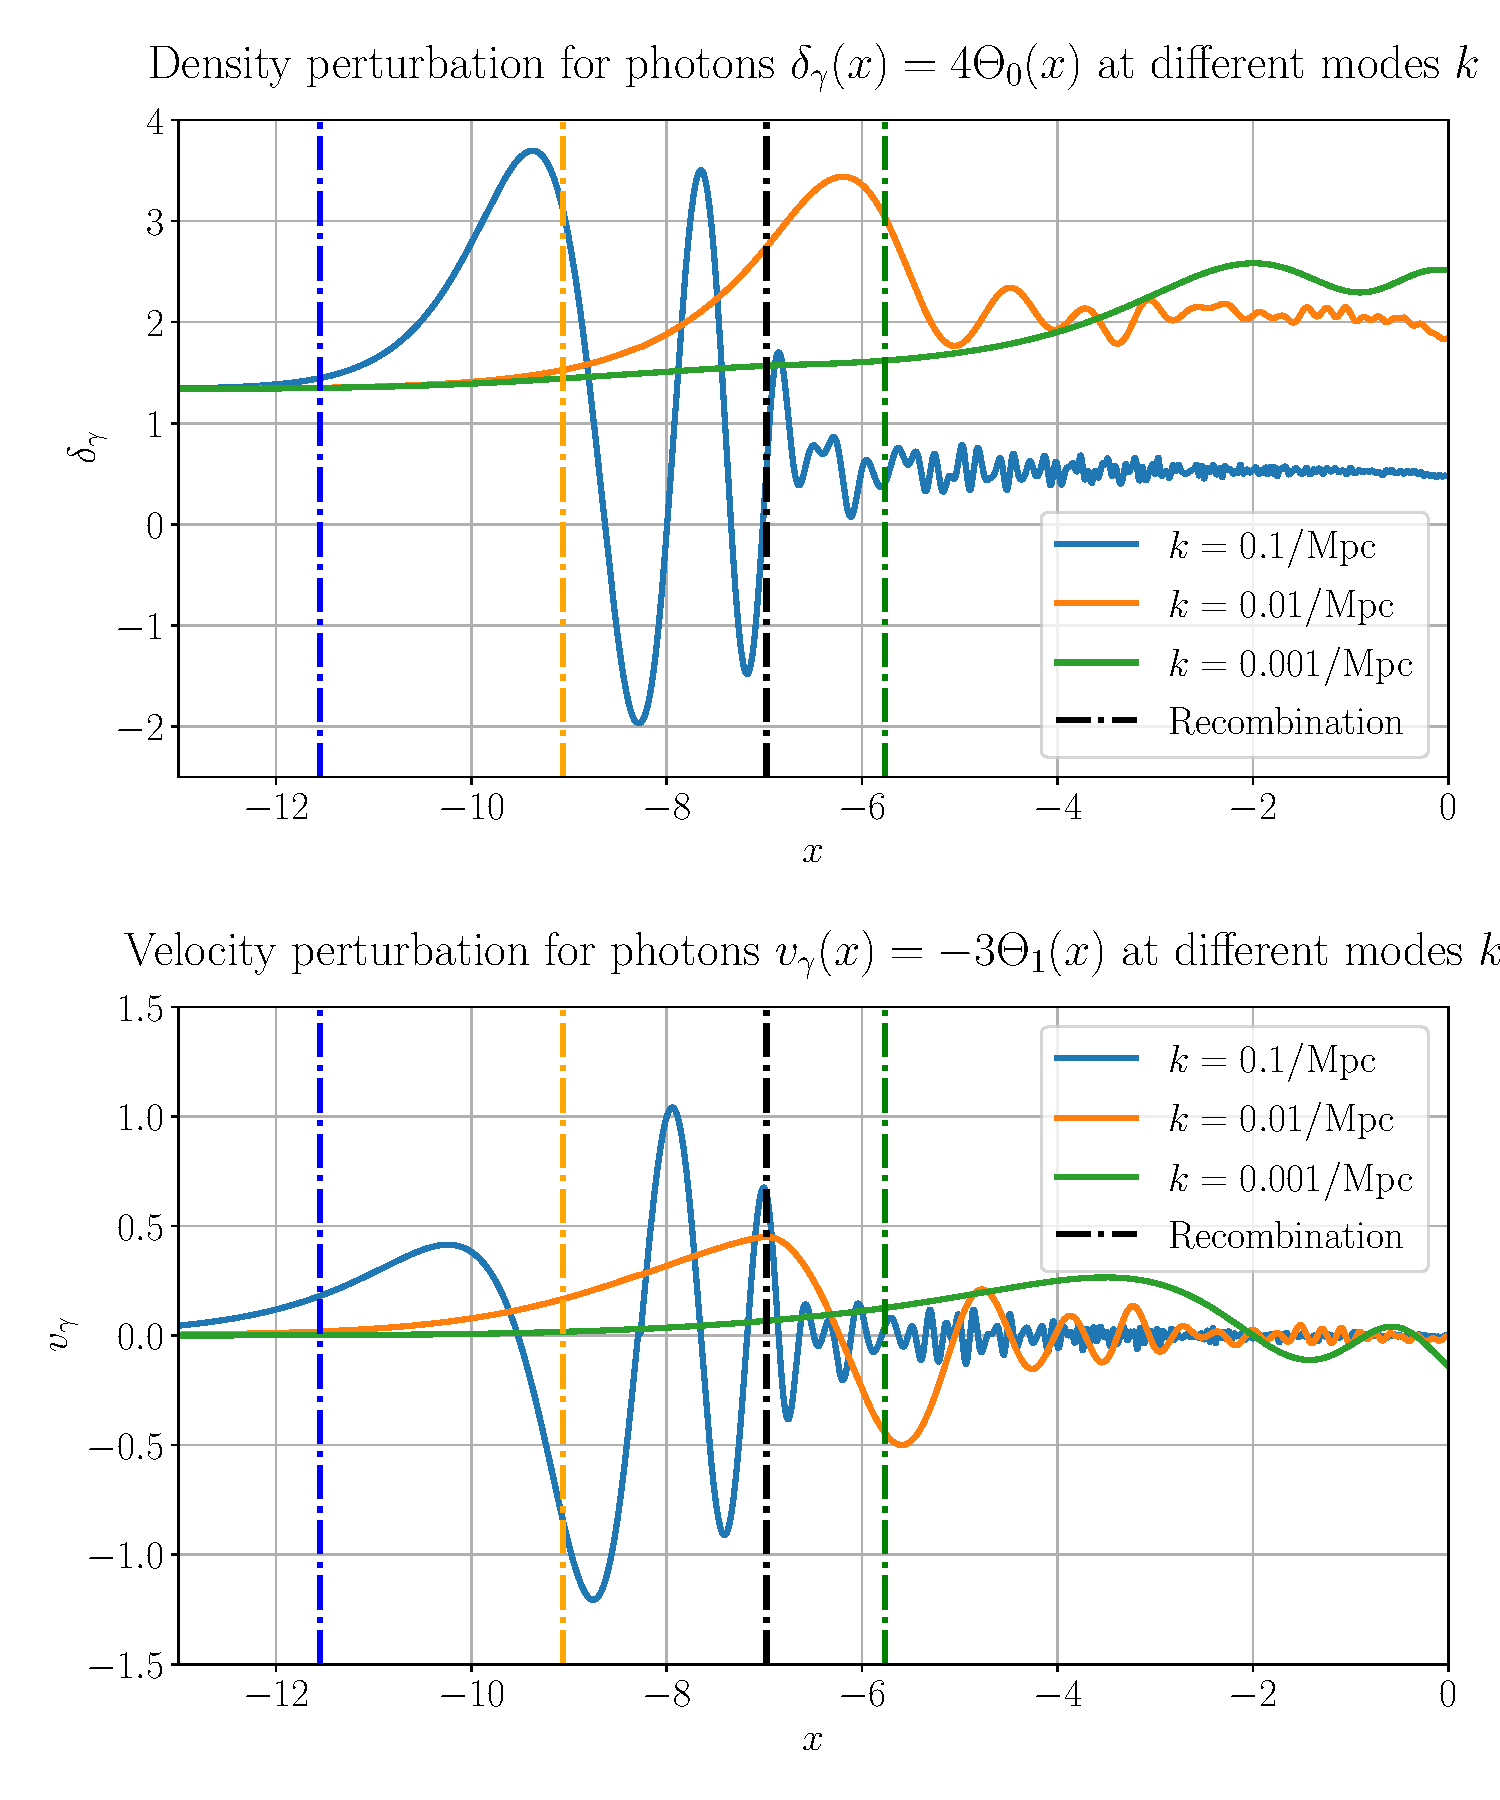
\includegraphics[width = \linewidth]{Figures/gamma.pdf}
	\caption{$\delta_\gamma$ and $v_\gamma$ as a function of $x$ at modes $k=0.1/\text{Mpc}$, $k=0.01/\text{Mpc}$ and $k=0.001/\text{Mpc}$ for small, intermediate and large scales respectively. The dot-dashed blue, yellow and green lines correspond to horizon crossing for the small, intermediate and large scale modes respectively and the black dot-dashed line corresponds to the time of recombination.}
	\label{fig:gamma}
\end{figure}

To gain a clearer understanding of the correlation between the overdensity and velocity of photons and baryons, Fig \ref{fig:gamma0.1}, \ref{fig:gamma0.01} and \ref{fig:gamma0.001} show $\delta_\gamma$ and $v_\gamma$ compared to $\delta_\text{B}$ and $v_\text{B}$ for the modes $k=\{0.1,0.01,0.001\}$/Mpc respectively. 

As expected from the discussion of the tight coupling regime, the two quantities are deeply related at all scales. Here one sees that even past the tight coupling regime, the two continue to follow one another at all scales, however the overdensities formed by the photons is noticeable larger at all scales. This can be seen from (\ref{eq:initial_conditions_pert}) as we begin with $\delta_\gamma=4\Theta_0=-2\Psi$, and $\delta_\text{B}=-\frac{3}{2}\Psi$ the ratio $\delta_\gamma/\delta_\text{B}=4/3$ exactly as we see in the figure at early times. 

\begin{figure}[ht!]
	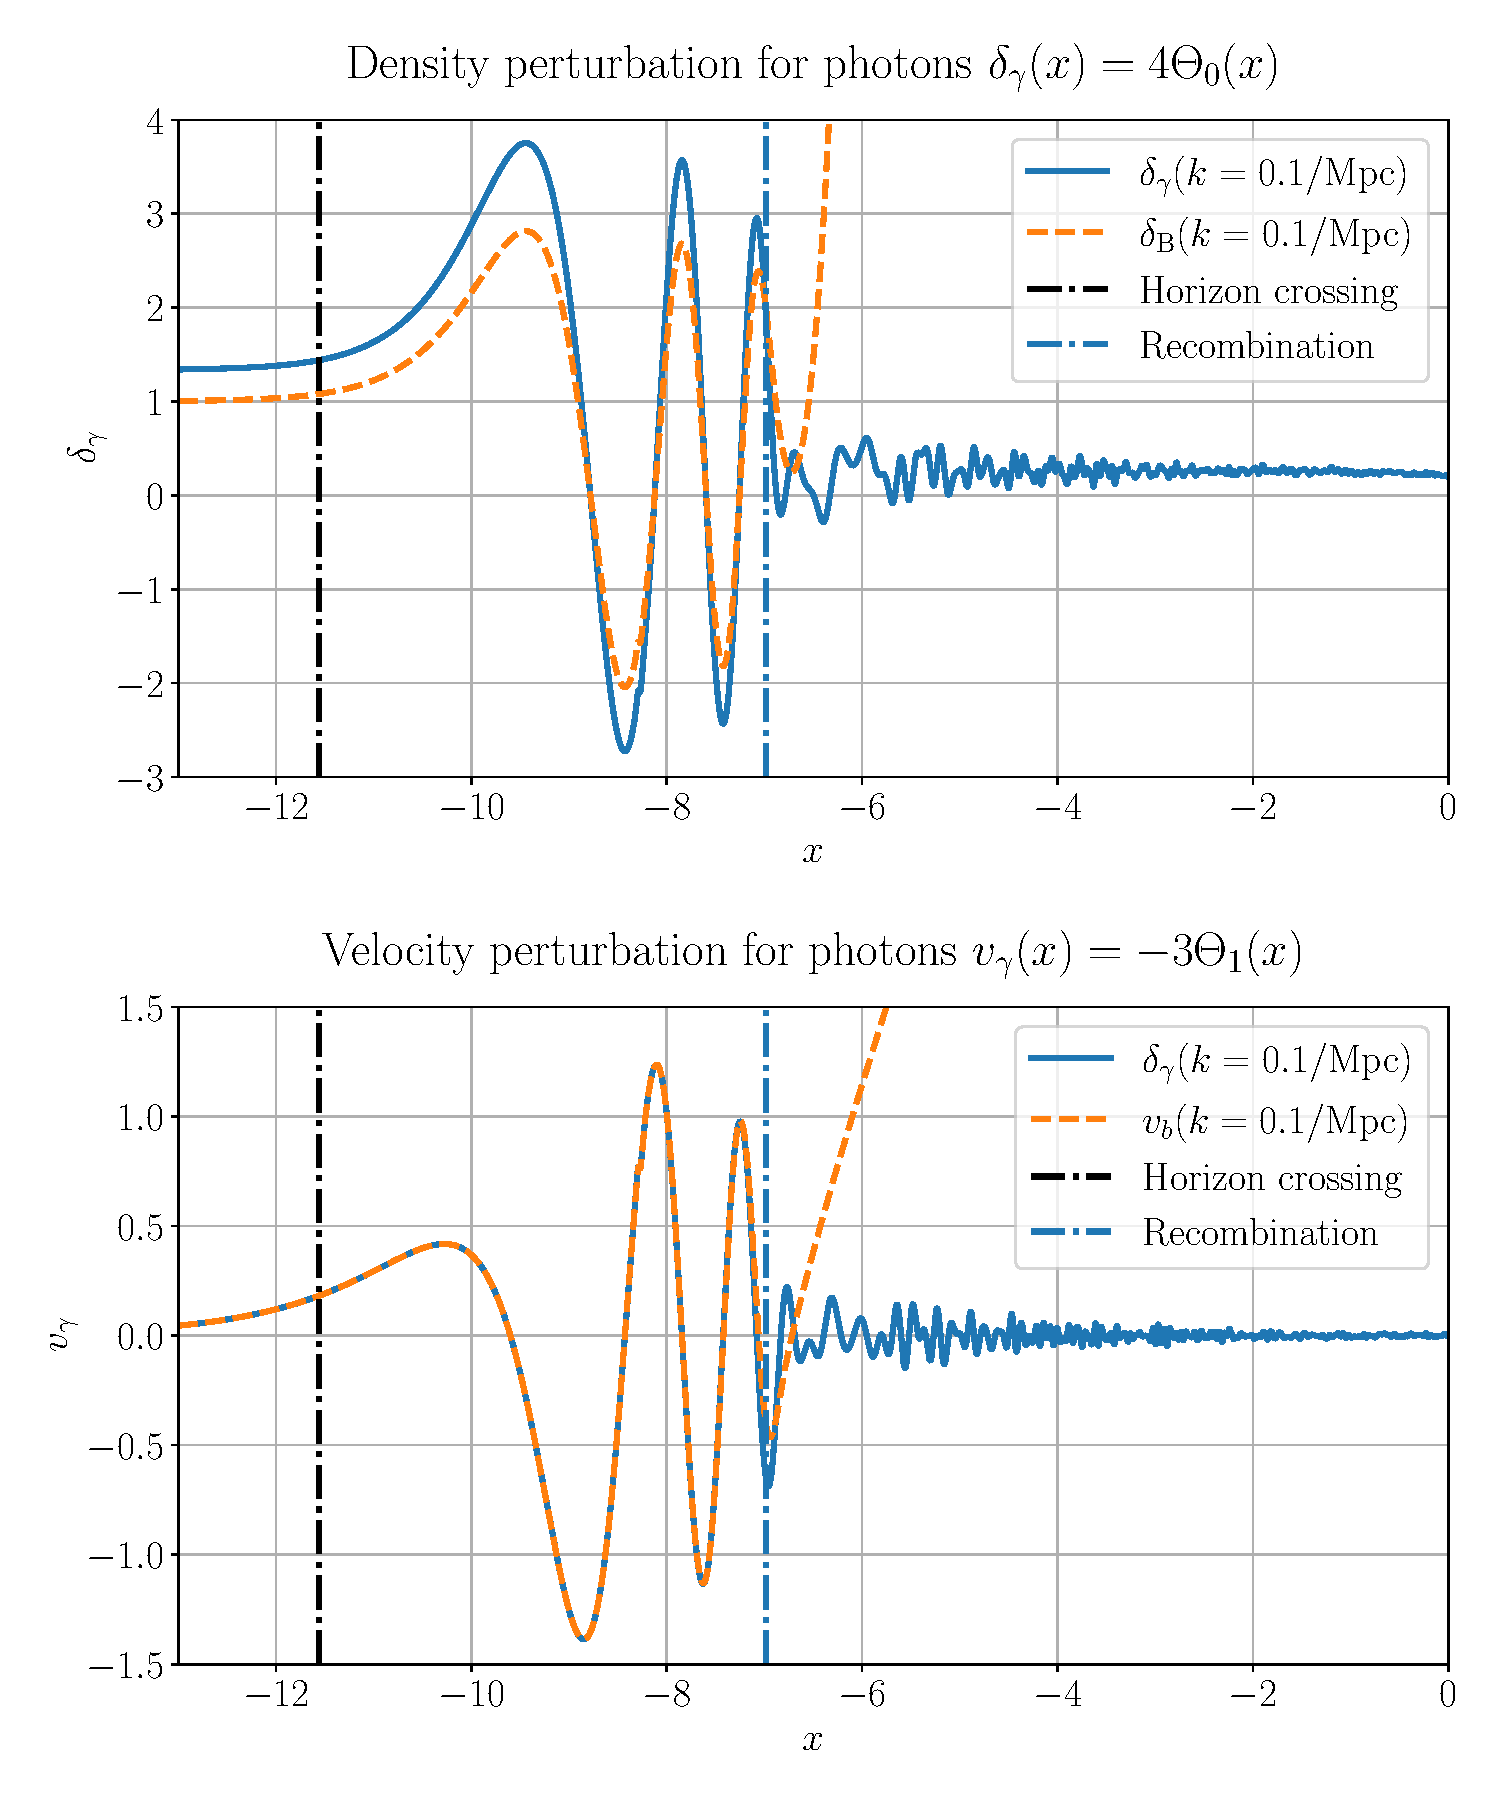
\includegraphics[width = \linewidth]{Figures/gamma0.1.pdf}
	\caption{$\delta_\gamma$ and $v_\gamma$ as a function of $x$ compared to $\delta_\text{B}$ and $v_\text{B}$ at the mode $k=0.1/\text{Mpc}$.}
	\label{fig:gamma0.1}
\end{figure}

For the smallest scale in depicted in Fig. \ref{fig:gamma0.1} one sees that after horizon crossing, the densities for both photons and baryons begin to grow due to gravitational wells. Later this reaches a peak as the radiation pressure causes an unstable equilibrium at around $x\approx-9.5$. This radiation pressure then drags the baryons along with the photons causing a propagation of the overdensity in the real space. At $x\approx-8.5$ the radiation pressure begins to be dominated by the gravitational wells caused by dark matter as previously discussed. This then continues a couple more times before recombination occurs. Once this happens, a near instantaneous decoupling between the photons and baryons can be seen, and baryons are left to freely cluster in the ever-growing gravitational wells. From here on the photons are effectively free as neutral atoms form and only experience mild oscillations about the average density fluctuations which we can clearly see is not at 0. Note that the effective photon temperature perturbation is in fact $\Theta_\text{eff}=\Theta_0+\Psi$ \cite{AST5220LectureNotes}. As such one does not expect the oscillations to oscillate about $0$ on these scales, but instead that $\Theta_\text{eff}$ does.
\begin{figure}[ht!]
	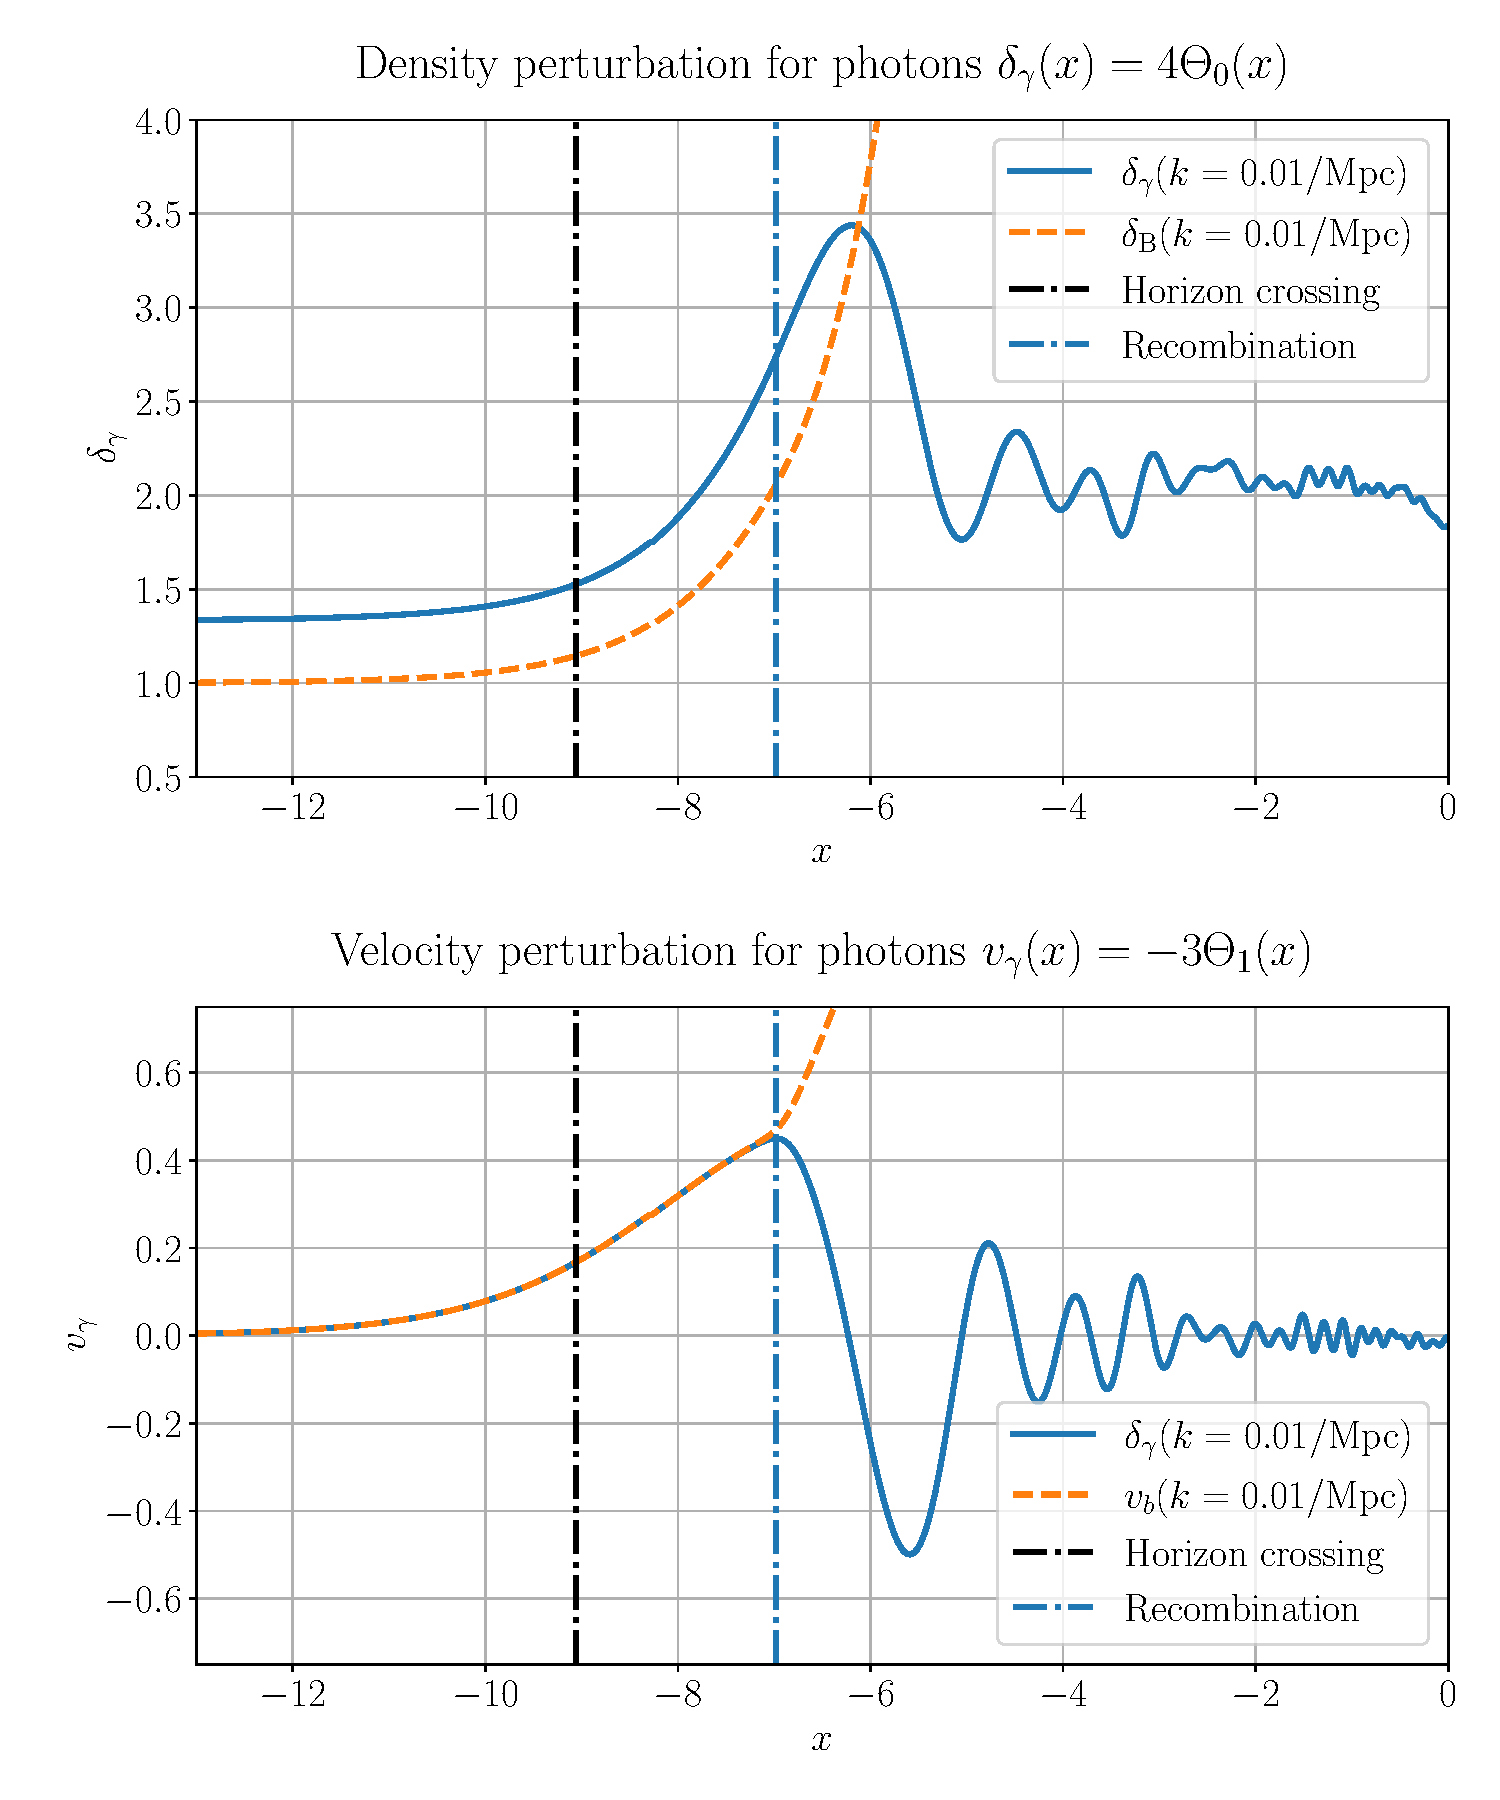
\includegraphics[width = \linewidth]{Figures/gamma0.01.pdf}
	\caption{$\delta_\gamma$ and $v_\gamma$ as a function of $x$ compared to $\delta_\text{B}$ and $v_\text{B}$ at the mode $k=0.01/\text{Mpc}$.}
	\label{fig:gamma0.01}
\end{figure}

In the intermediate scale shown in Fig. \ref{fig:gamma0.01} we again see much of the same physics as for the smallest scale. As in the discussion for the baryons and CDM, the clustering begins to manifest shortly before the horizon crossing. Here one can more readily see that the clustering occurs until a bit after recombination, but does not have time to cause the oscillatory motion for the baryons that we saw on the smallest scale. The photon density then dips down again until it reaches its equilibrium. Note that when the Universe begins to accelerate, a noticeable second dip in the photon density occurs. This is once again due to dark energy domination occurring and is more prominent on larger scales.

\begin{figure}[ht!]
	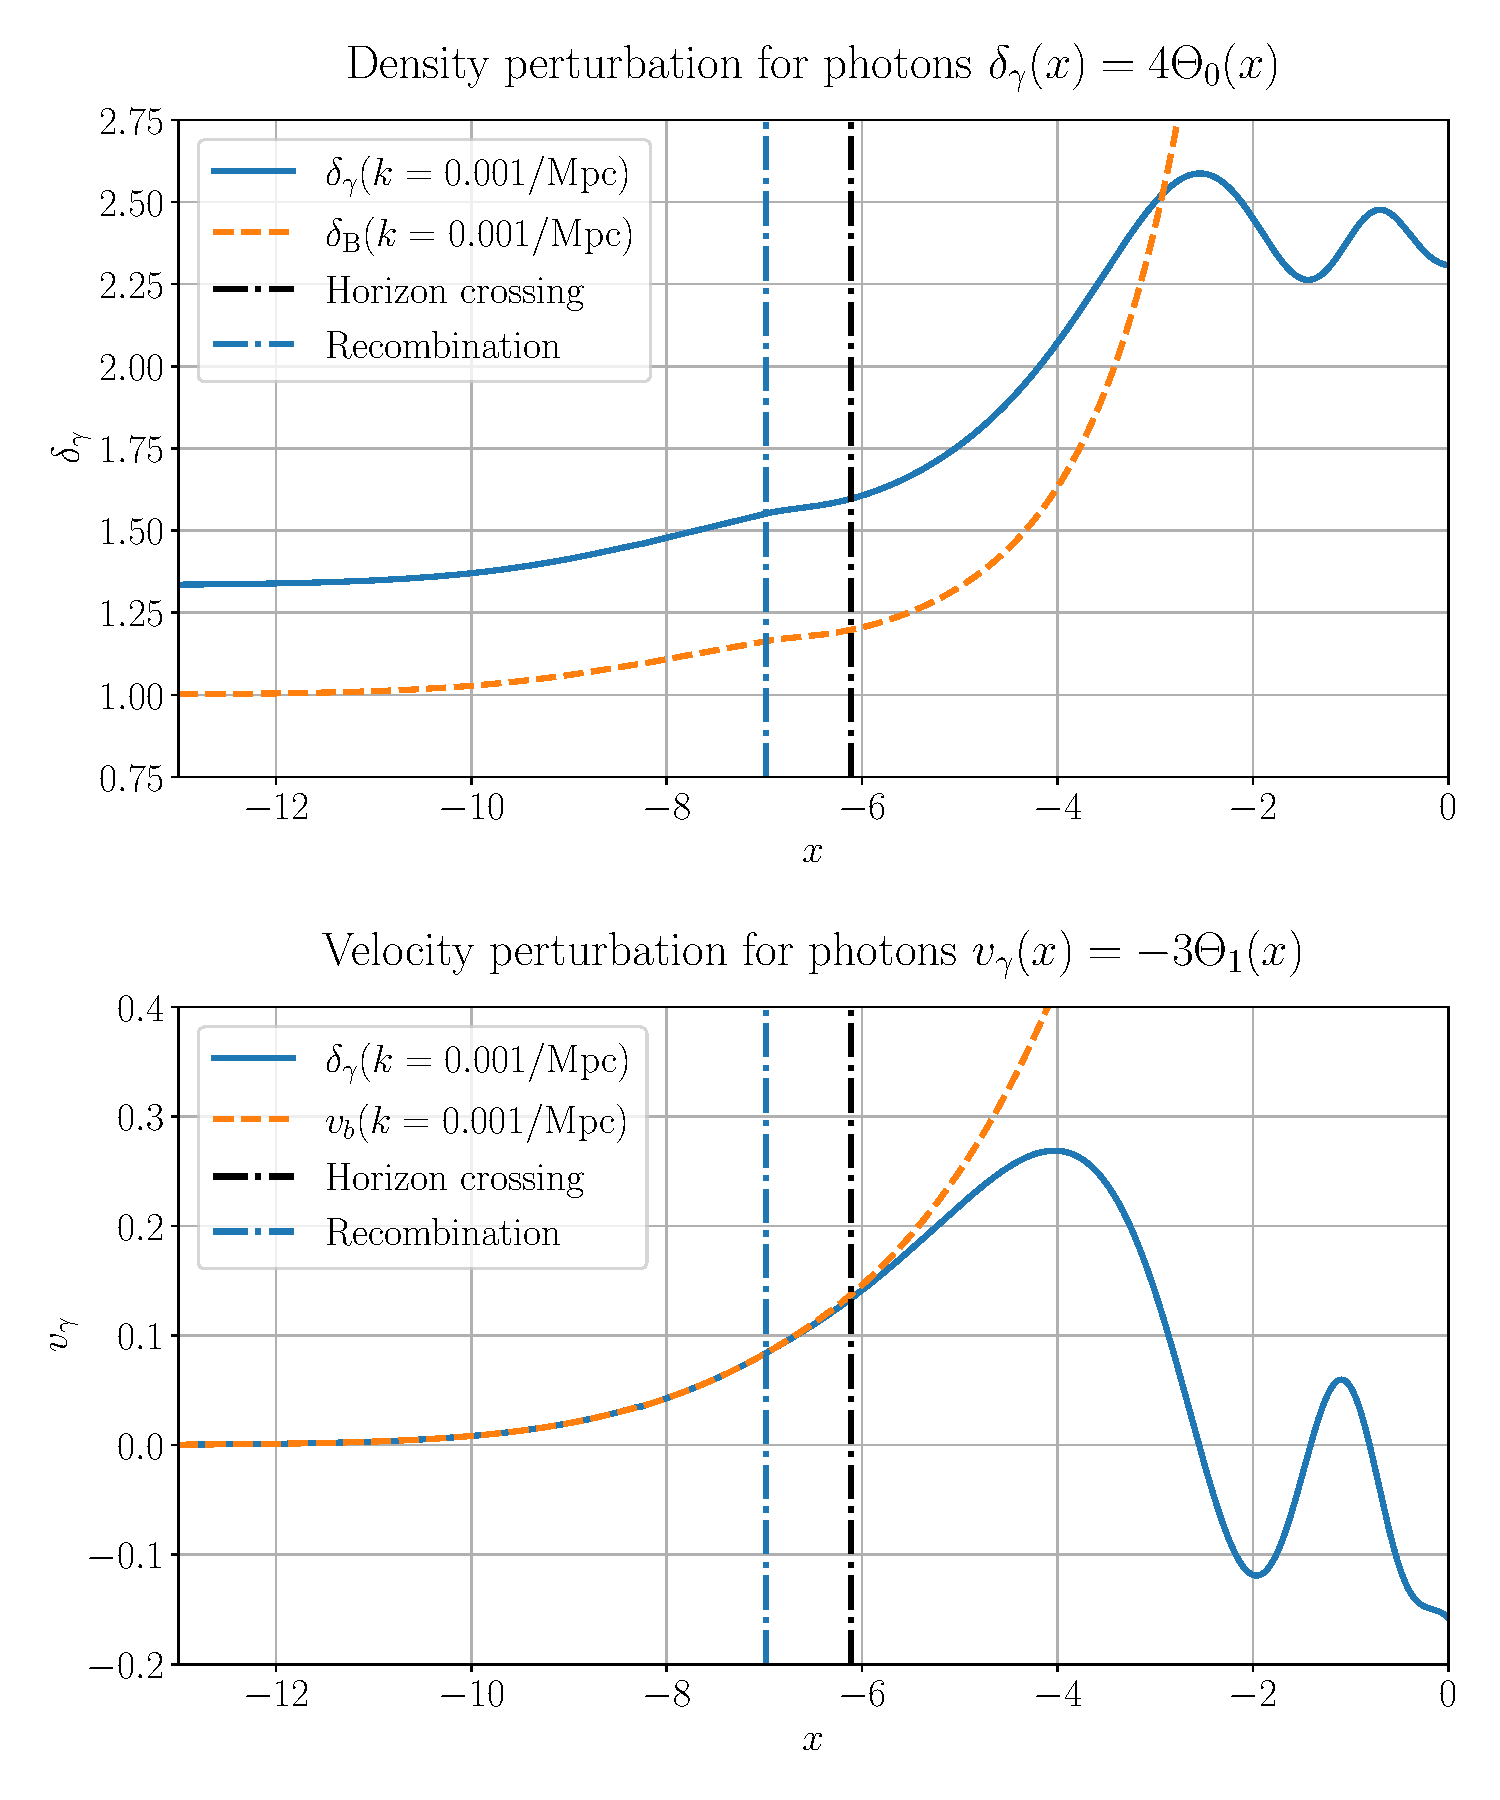
\includegraphics[width = \linewidth]{Figures/gamma0.001.pdf}
	\caption{$\delta_\gamma$ and $v_\gamma$ as a function of $x$ compared to $\delta_\text{B}$ and $v_\text{B}$ at the mode $k=0.001/\text{Mpc}$.}
	\label{fig:gamma0.001}
\end{figure}

The largest scale that we consider in Fig. \ref{fig:gamma0.001} the build-up starts much later. Unlike the prior two scales, the velocities of the baryons and photons do not immediately decouple to the same extent after recombination at these scales. But we can still see that there is a noticeable difference in the two past this point. The oscillations in Fourier space after the photon density peak is then much slower here compared to the previous cases due to the propagating waves travelling at velocity $\sim c$ in real space moving much slower relative to the size of the scale.

Next we consider the evolution of the quadrupole moment $\Theta_2$ for the considered length scales depicted in Fig. \ref{fig:T2}.

\begin{figure}[ht!]
	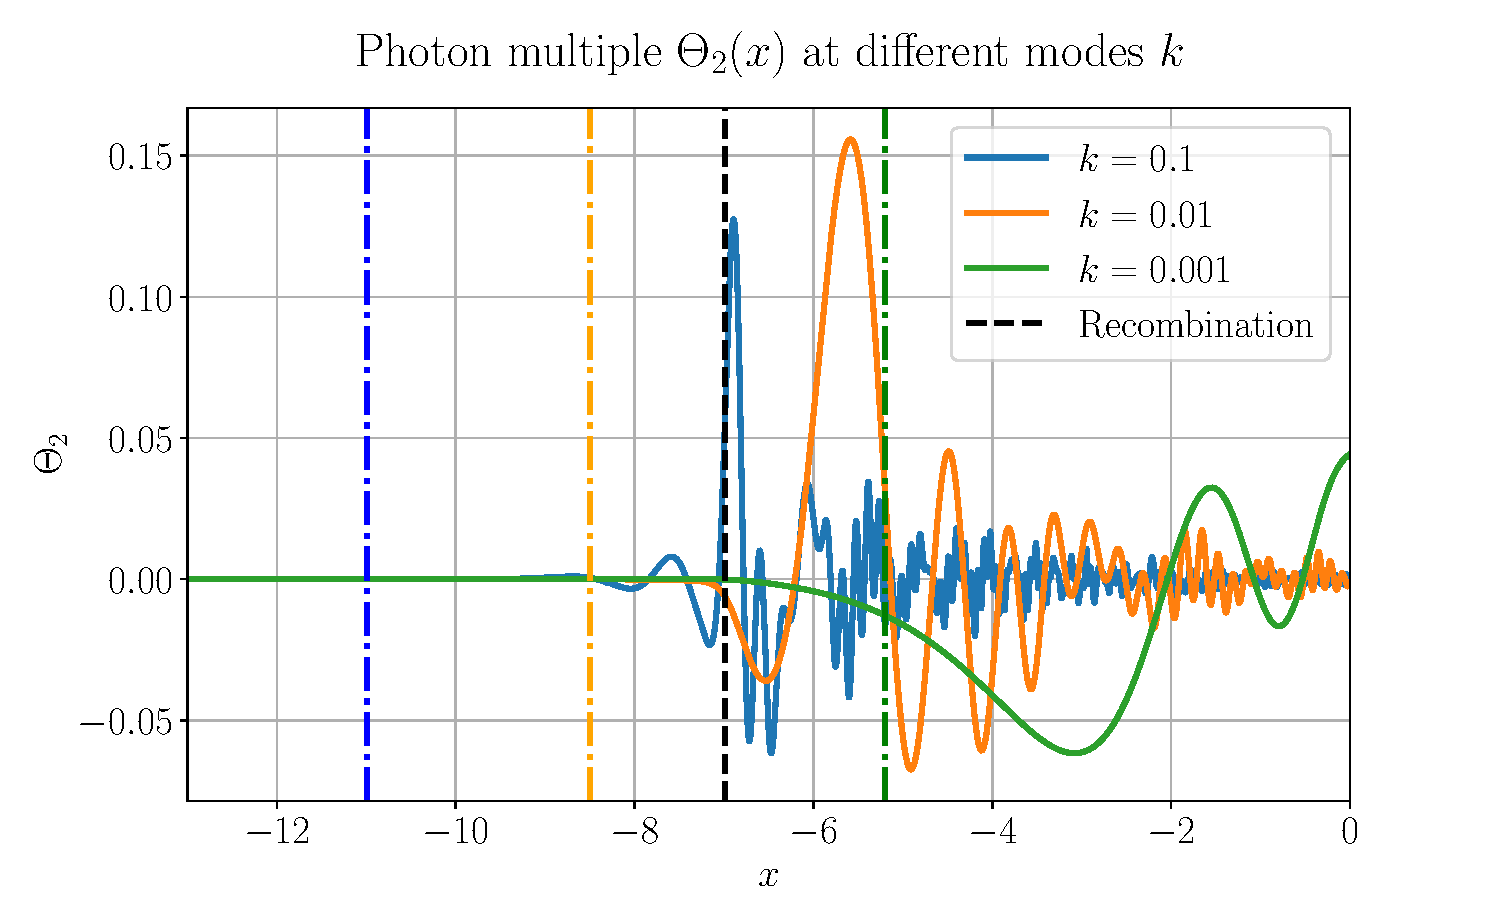
\includegraphics[width = \linewidth]{Figures/Theta2.pdf}
	\caption{Time evolution of the photon quadrupole $\Theta_2$ at modes $k=0.1/\text{Mpc}$, $k=0.01/\text{Mpc}$ and $k=0.001/\text{Mpc}$ for small, intermediate and large scales respectively. The dot-dashed blue, yellow and green lines correspond to horizon crossing for the small, intermediate and large scale modes respectively.}
	\label{fig:T2}
\end{figure}

One thing to note is that in the derivation of the TC system, an assumption that the early Universe is without anisotropic stress, meaning that the stress energy tensor is invariant under spatial rotations. As a consequence, given our conventions, the EFE sets $\Phi=-\Psi$. In the full system this is however not necessarily the case. With this in mind, considering (\ref{eq:metric_perturbations_final}b), we see that in this model, anisotropic stress in then deeply related to both $\Omega_\gamma$ and $\Theta_2$. In the era where $\Theta_2=0$ we will then expect the sum $\Phi+\Psi=0$ which we will come back to later. 

For the smallest scale we see that the oscillations in Fourier space begin quite late in comparison to when one would expect to see effects due to the horizon crossing. A small oscillation can then be seen to build up rather quickly until it peaks shortly after recombination. As such the anisotropy that one would expect from photons in the CMB spectra should be rather large at these scales. This also implies that the assumption that $\Phi=-\Psi$ is less convincing at this time, something that we will see later. The oscillations then quickly fall off as time evolves past recombination, but are still noticeable compared to before TC ends.

For the intermediate scale we see that the oscillations begin much faster when compared to the particle horizon. As in the small scale the oscillations quickly build up, peaking at about $x\approx-5.5$. This once again signifies anisotropies. As with the small scales, the oscillation decay, but albeit at a much slower pace.

At the largest scale we see that the main oscillation starts up before the expected horizon crossing. It then has its absolute extremum at $x\approx-3.5$ and continues its oscillatory motion until present day.


\subsubsection{Gravitational potentials}
Considering the potentials $\Phi$ and $\Psi$ as a function of time for the modes $k=\{0.1,0.01,0.001\}$/Mpc shown in Fig. \ref{fig:phi_psi} where the potential $\Phi$ is given in the top figure and the sum $\Phi+\Psi$ is given in the lower figure. 
\begin{figure}[ht!]
	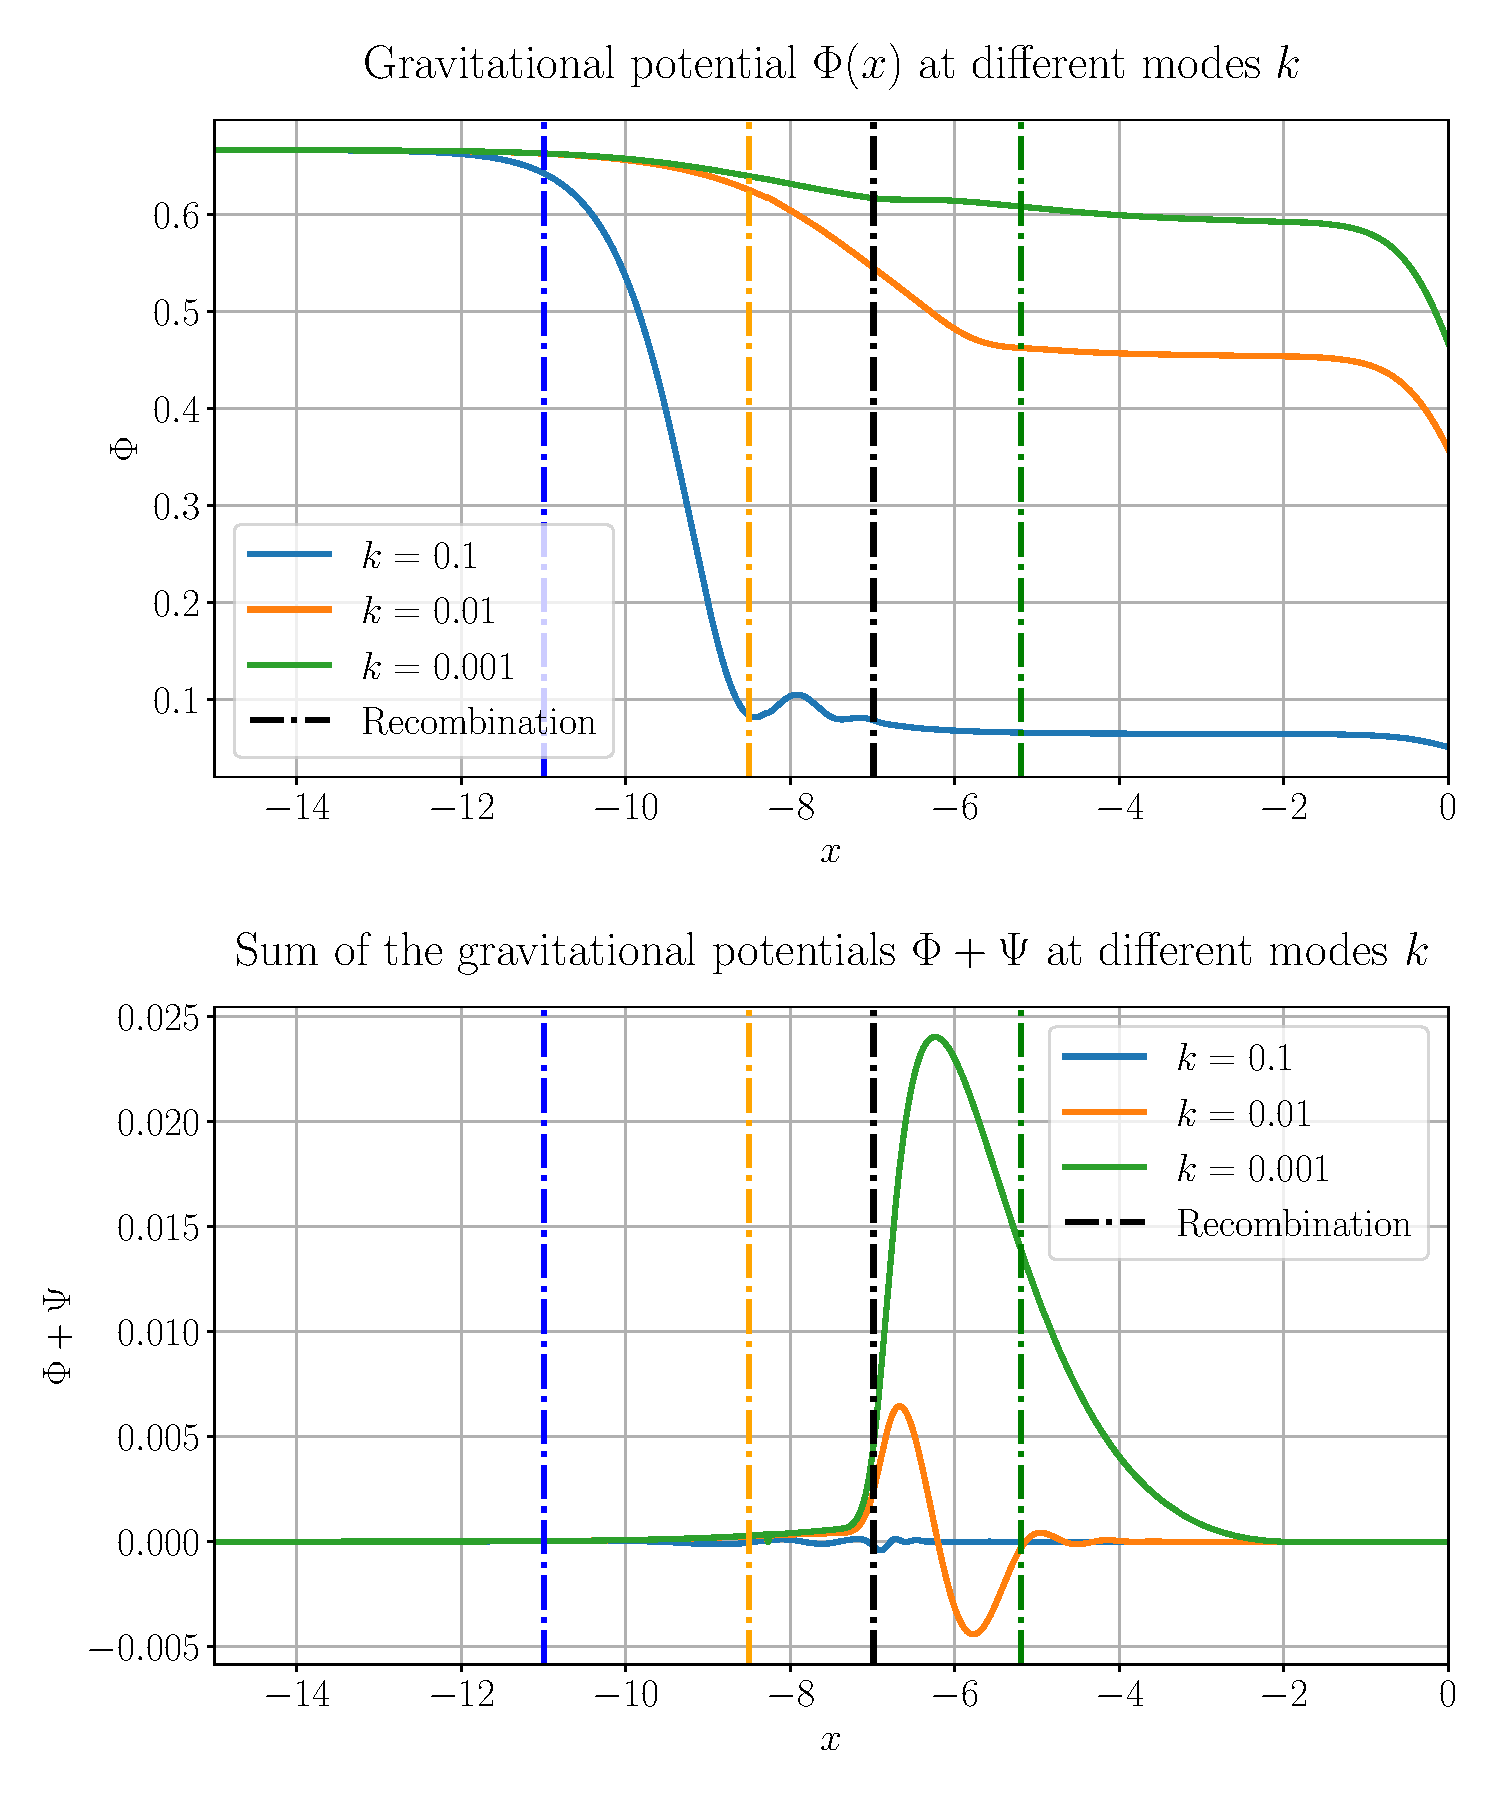
\includegraphics[width = \linewidth]{Figures/Phi_Psi.pdf}
	\caption{Time evolution of $\Phi(x)$ along with the sum $\Phi(x)+\Psi(x)$ at modes $k=0.1/\text{Mpc}$, $k=0.01/\text{Mpc}$ and $k=0.001/\text{Mpc}$ for small, intermediate and large scales respectively. The dot-dashed blue, yellow and green lines correspond to horizon crossing for the small, intermediate and large scale modes respectively.}
	\label{fig:phi_psi}
\end{figure}

At early times we see that the potential $\Phi$, and thus the potential $\Psi$ are constant as expected due to the horizon being much smaller than the considered modes. As can be seen from the second figure, $\Phi=-\Psi$ at early times justified by the fact that the quadrupole moment $\Theta_2=0$ at this time.

At later times, as the particle horizon expands, the smaller scales, corresponding to the higher value of the modes, enter the horizon. As indicated in Table \ref{tab:ketasim1} for small scales, it is expected that causal physics will begin to play a role at around $x\approx -11.0$. In turn this allows for radiation pressure, which is dominant at this time, to effectively counteract the gravitational potential and prevents over-densities to form in the primordial baryon-photon plasma. After a large drop in $\Phi$, it then begins to oscillate in a damped fashion which comes from the back-and-forth between radiation pressure and induced gravitational wells from CDM and baryons. This is clearly seen at smaller scales but the effect is massively suppressed at larger scales. One can also notice that the sum $\Phi+\Psi$ barely changes at these small scales, suggesting that the anisotropies at these scales are relatively small, but there are still some small oscillations around recombination as could be expected from Fig. \ref{fig:T2}. Finally the potential $\Phi$ flattens out during matter domination, which is to be expected for $k\gtrsim0.1$/Mpc which agrees with our result. 

For the intermediate scales we see that the drop-off of the potential starts later, once again expected from Table \ref{tab:ketasim1} and is much slower compared to smaller scales. This is due to the mode entering the horizon during the transition between radiation and matter domination. The drop-off then remains constant with respect to $x$ during recombination until, as before, it flattens out to a constant during matter domination. The anisotropies, in the lower figure, are noticeable at these scales. 

The large scale mode begins to drop at roughly the same time as intermediate scales, but once again slower than the others. Table \ref{tab:ketasim1} seems to imply that this cannot causally happen at this time. However this is not due to gravitational interactions at this time, but instead due to the transition to radiation domination. Analytically one can find the expected change to the potential to be a factor of $9/10$ as this transition occurs \cite{AST5220LectureNotes} which seems to agree with the green line in the top figure. Further there is a much larger relative difference between the two potentials, due to the $k^{-2}$ dependence in the anisotropy term.

For all scales we see that during matter domination, the gravitational potentials flatten out at every scale. Naively one would expect it to increase in this period as all matter is effectively neutral and thus things would collapse together gravitationally, but the expansion of the Universe works as a counteractive force against gravitational wells, and thus it remains roughly constant at all scales. In the lower figure we see that at late times the sum of the Newtonian scalars once again satisfy $\Phi=-\Psi$. Again referring (\ref{eq:metric_perturbations_final}b) we have that $\Omega_\gamma\approx0$ past a certain point. As such, even with the continuing oscillatory motion of the quadrupole moment, the anisotropies are cancelled out by the lack of radiation at late times.  At last one sees a drop-off, where the magnitude of this drop-off is seemingly proportional to the scale, as the Universe begins to expand due to dark energy beginning to dominate. This makes sense physically as when the repulsive nature of dark energy takes over, it will expand the distance between massive objects, causing the gravitational potentials to fall off.

\subsection{Summary}
In this section we first solved the approximated tight coupling system and exited this system before our approximations broke down. We then switched over to the full system up to the given $\ell_\text{max}=7$. Three particular modes, each representing a given scale, were then chosen and discussed in detail for the various quantities. 

\end{document}